\section{Die Berechnung des Kohlebedarfs}

Im Folgenden wird erläutert, wie aus Stromproduktionsdaten der Kohlebedarf für ein Kraftwerk berechnet wird. Außerdem wird erklärt, wie daraus Abfahrtszeiten für Kohlezüge bestimmt werden können. Viele Informationen dieses Abschnittes, welche mit dem Kohleverkehr in der Lausitz in Zusammenhang stehen, stammen aus einem Interview mit Sascha Lesche von der LEAG (siehe Anhang Eins). Abbildung \ref{fig:demand-calculation} zeigt den Ablauf dieser Berechnung.

\begin{sidewaysfigure}[htb]
	\centering
	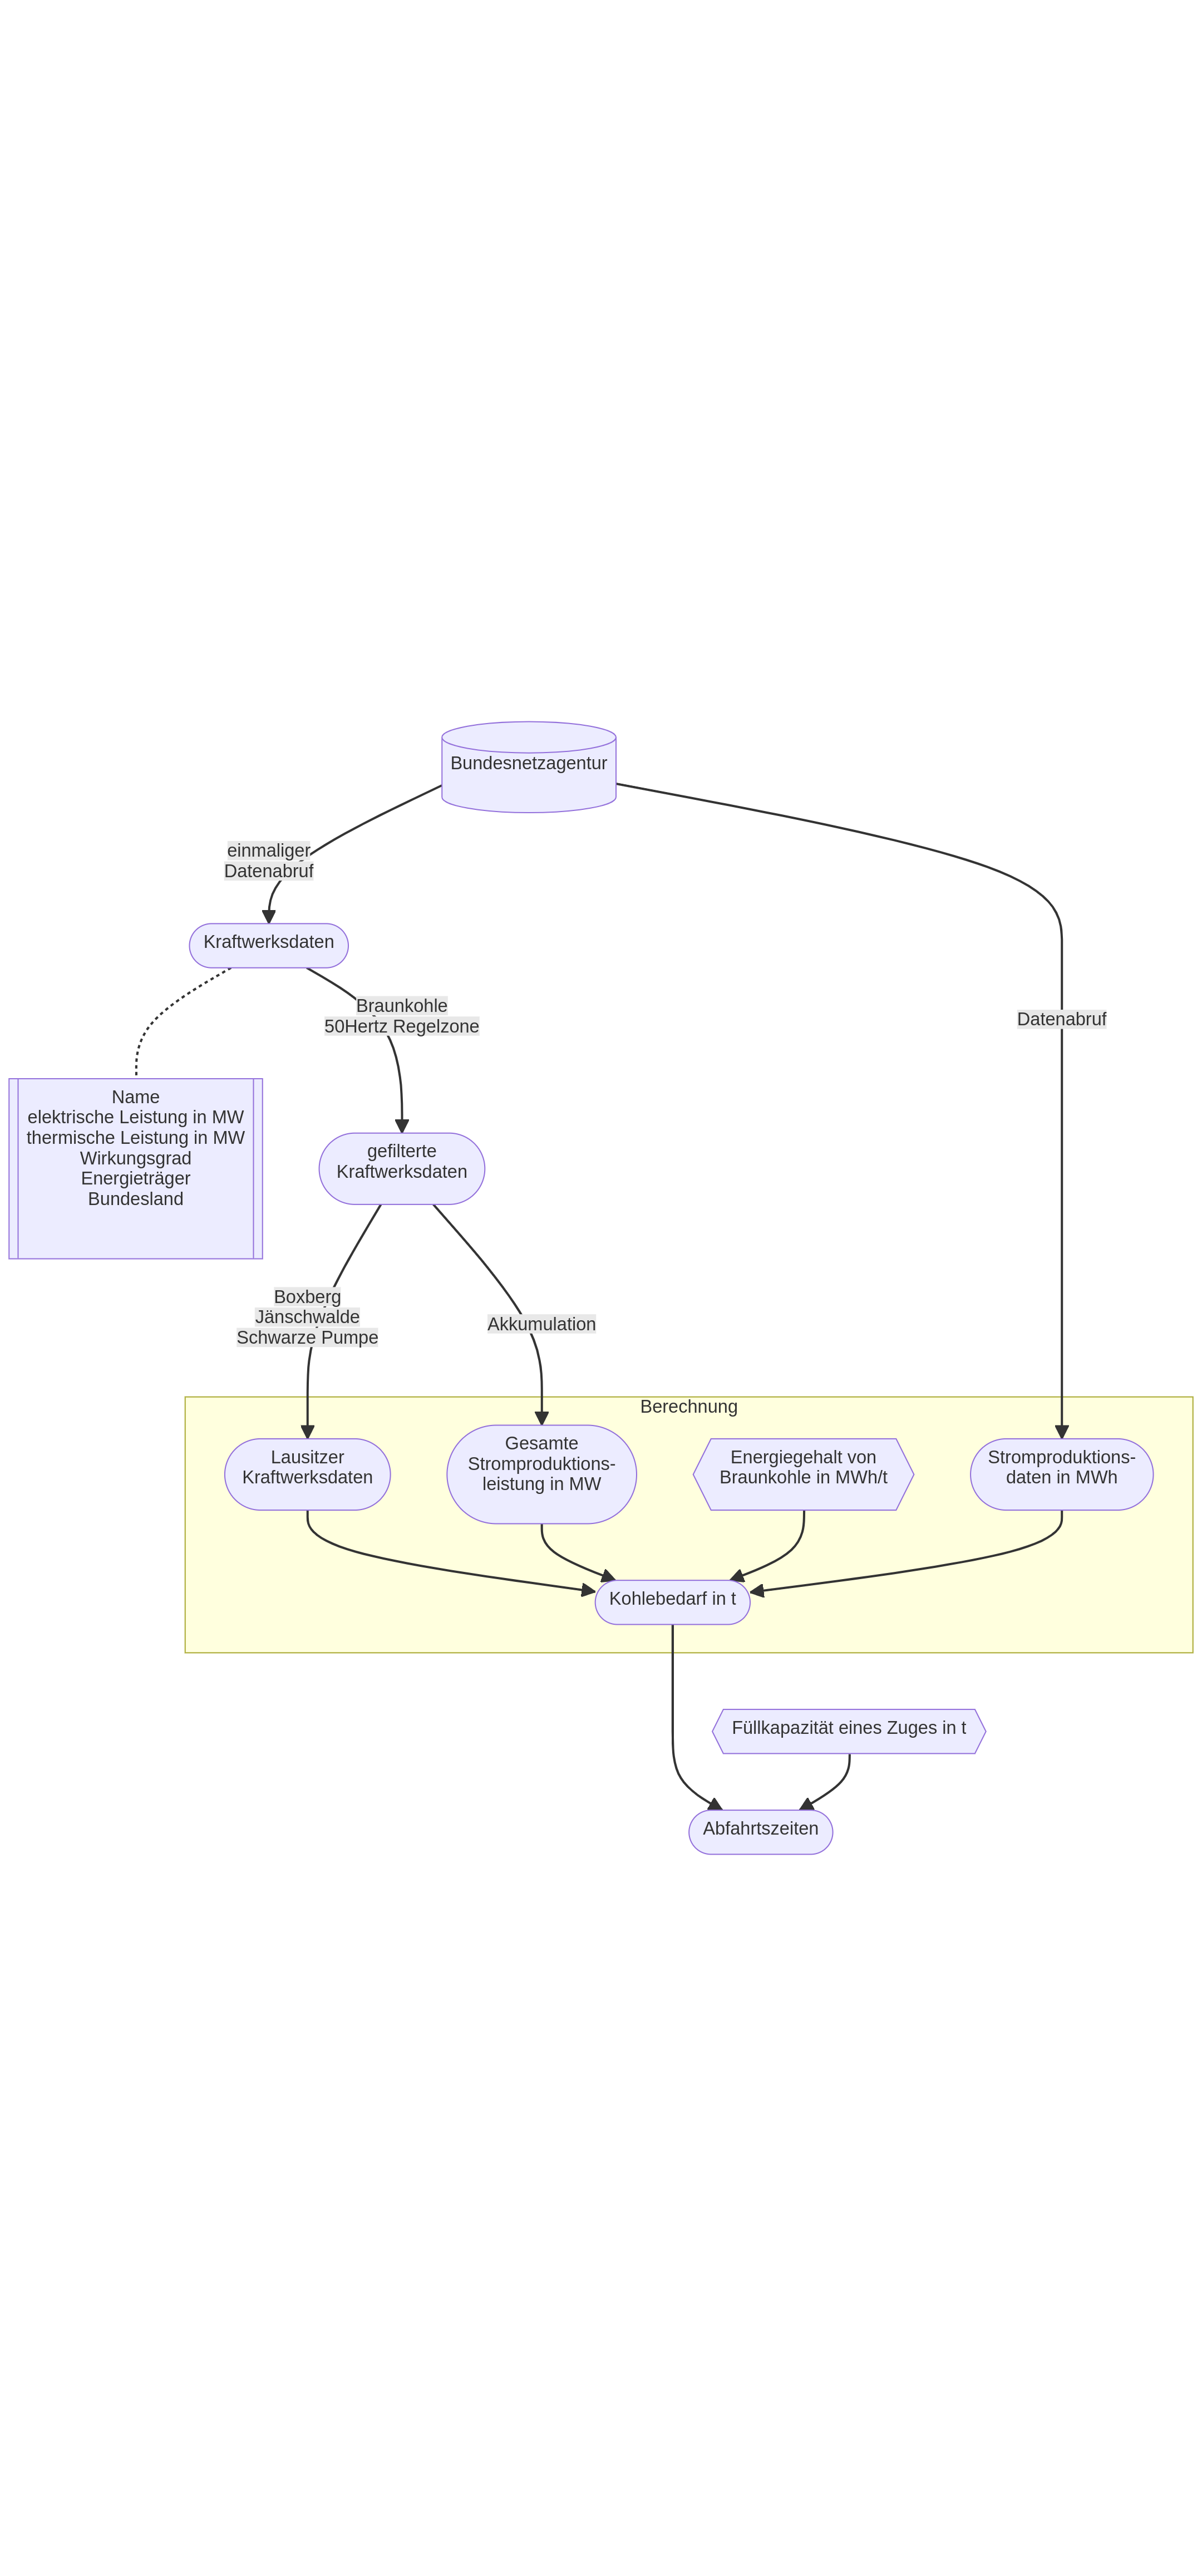
\includegraphics[width=1.0\linewidth]{images/diagrams/demand-calculation.png}
	\caption{Schematische Abbildung der Berechnung des Kohlebedarfs eines Kraftwerkes und der benötigten Anzahl an Kohlezügen aus Stromproduktionsdaten und Kennzahlen von Kraftwerken. Der Zylinder stellt eine Datenquelle dar, die abgerundeten Felder Daten und die Hexagone Konstanten.}
	\label{fig:demand-calculation}
\end{sidewaysfigure}

Die Bundesnetzagentur stellt Kenndaten zu allen Kraftwerken Deutschlands bereit\cite{noauthor_bundesnetzagentur_nodate}. Die für uns wichtigen Kraftwerksdaten sind der Name des Kraftwerkes, seine elektrische Leistung in MWh, die thermische Leistung in MW, der verwendete Energieträger und das Bundesland, ich welchem sich das Kraftwerk befindet. Diese Daten wurden einmalig in Form einer CSV-Datei heruntergeladen. Im Anschluss wurden die Daten gefiltert, sodass nur noch Kraftwerke mit dem Energieträger Braunkohle innerhalb der \emph{50Hertz}-Regelzone übrige blieben. Diese Zone umfasst die neuen Bundesländer und Hamburg. Aus diesen gefilterten Kraftwerksdaten wurde dann die Gesamtleistung $P_T$ aller Braunkohlekraftwerke in der Regelzone durch Aufsummieren berechnet. Diese Gesamtleistung beträgt rund 10.600 MW. Außerdem wurden für die weitere Berechnung nur noch die drei Lausitzer Kraftwerke betrachtet, welche über das Schienennetz der LEAG mit Braunkohle versorgt werden. Diese Kraftwerke sind \emph{Boxberg}, \emph{Jänschwalde} und \emph{Schwarze Pumpe}.\\
\\
Die produzierte Energiemenge $E$ aus Braunkohle in der 50Hertz-Regelzone für einen bestimmten Zeitraum kann von der Smard-API abgerufen werden. Unter der Annahme, dass alle Kraftwerke dieser Zone gleichmäßig ausgelastet werden, benötigen sie eine Zeitspanne von $\Delta t$, um die Energiemenge $E$ zu produzieren. $\Delta t$ ergibt sich, wie in Formel \ref{eq:energy-time} dargestellt, aus dem Quotienten aus der produzierten Energie und der Gesamtleistung aller Kraftwerke.

\begin{equation}
    \Delta t = \frac{E}{P_T}\label{eq:energy-time}
\end{equation}

Die benötigte Kohlemenge $m_k$, die ein Kraftwerk benötigt, um $\Delta t$ lang bei voller Leistung Strom zu produzieren, kann mit Hilfe von Formel \ref{eq:coal-mass} berechnet werden. Dabei sind $P_e$ die elektrische Leistung und $P_t$ die thermische Leistung des betrachteten Kraftwerkes in MW. Weiterhin sind $\rho$ die mittlere Energiedichte von Braunkohle mit 5,56 MWh/t \cite{paschotta_kohle_2023} und $\eta$ der Wirkungsgrad des Kraftwerkes.

\begin{equation}
    m_k=\frac{\Delta t(P_e+P_t)}{\rho\eta}\label{eq:coal-mass}
\end{equation}

Zusammen mit der Füllkapazität eines Kohlezuges $c$ von 960 t lässt sich durch Formel \ref{eq:train-amount} die Anzahl der Züge $n_z$ berechnen, die benötigt wird, um die Masse an Kohle zu transportieren.

\begin{equation}
    n_z=\frac{m_k}{c}\label{eq:train-amount}
\end{equation}

Die Anzahl an Zügen kann dann über die Zeit akkumuliert werden, sodass immer wenn dieser Wert eine ganze Zahl überschreitet, ein Zug abfahren kann.\\
\\
Die für diese Berechnung verwendeten Annahmen sind die Folgenden:
\begin{itemize}
    \item Alle Kraftwerke der \emph{50Hertz}-Regelzone werden gleichmäßig (gewichtet mit ihrer jeweiligen Maximalleistung) ausgelastet.
    \item Das Verhältnis zwischen elektrischer Leistung $P_e$ und thermischer Leistung $P_t$ eines Kraftwerkes ist konstant.
    \item Der Wirkungsgrad eines Kraftwerkes ist eine Konstante und nicht abhängig von der momentan bereitgestellten Leistung.
\end{itemize}
Diese Annahmen mussten getroffen werden, da keine Daten mit höherer räumlicher Auflösung zur Verfügung standen und das Leistungsverhalten eines Kohlekraftwerkes für unsere Zwecke vereinfacht wurde. Die Güte bzw. der Realismus dieser Annahmen wird sich letztendlich aus dem Vergleich der Simulationsergebnisse mit Referenzdaten ergeben.
